%!TEX root = ../../common/main.tex

\section{Decay time resolution and acceptance}
\label{sec:measurement_of_sin2beta:resolution_and_acceptance}

In the following sections the influence of the decay time resolution and
acceptance effects are studied. 

% ------------------------------------------------------------------------------
\subsection{Resolution}
\label{sec:measurement_of_sin2beta:resolution_and_acceptance:resolution}
\missing{Decay time resolution}

% ------------------------------------------------------------------------------
\subsection{Decay time acceptance}
\label{sec:measurement_of_sin2beta:resolution_and_acceptance:acceptance}

Acceptance effects that alter the distribution of the decay time might result
from selection requirements or inefficiencies in the event reconstruction.
\Cref{sec:measurement_of_sin2beta:resolution_and_acceptance:acceptance:lower}
summarises acceptance effects stemming from lifetime biasing selection cuts from
the trigger requirements
(\cf \cref{sec:measurement_of_sin2beta:data_preparation:trigger}). Reconstruction
inefficiencies mainly caused by the \VELO track reconstruction algorithms (\cf
\cref{sec:lhcb_experiment:tracking}) are outlined in
\cref{sec:measurement_of_sin2beta:resolution_and_acceptance:acceptance:upper}.

% ..............................................................................
\subsubsection{Trigger induced decay time acceptance}
\label{sec:measurement_of_sin2beta:resolution_and_acceptance:acceptance:lower}

The biased trigger lines (\cf
\cref{sec:measurement_of_sin2beta:data_preparation:trigger}) and the stripping
cut on the reconstructed decay time of the $\Bd$ candidates result in a non-flat
acceptance. A data driven method is used to determine and to describe this
effect.

In order to correctly describe these effects, the data sample is split into two
disjoint categories of candidates that show a substantially different behaviour
regarding their decay time acceptance. All candidates passing the \emph{almost
unbiased} (\textbf{\catAU}) trigger requirements show nearly no decay time
acceptance effects, in contrast to the sample of candidates passing the
\emph{exclusively biased} (\textbf{\catEB}) trigger requirements. The addressed
requirements are:
%
\begin{description}
  \item[\catAU] \TriggerReqAU
  \item[\catEB] \TriggerReqEB
\end{description}
%
To construct the acceptance in terms of ratios, a sample of candidates that pass
a set of unbiased trigger requirements is needed:
%
\begin{description}
  \item[Unbiased] \TriggerReqUB
\end{description}
%
The acceptance of the \catAU subsample can be computed using the overlap of events
which pass both the \HLTTwoDiMuonDetachedJpsi and the
\HLTTwoDiMuonJpsi line. Both lines are using the same trigger cuts except for
an additional cut on the flight distance significance (see
\cref{tab:measurement_of_sin2beta:data_preparation:trigger:hlt2:cuts}) in the
case of the biased lines. The acceptance can then be written as a time-dependent
efficiency $\varepsilon_\text{\catAU}$, with
%
\begin{equation}
  \begin{split}
    \varepsilon_\text{\catAU} &= \frac{\VerbAU \VerbAnd \HLTTwoDiMuonJpsi}{\VerbUB}\\
                              &= \frac{\TriggerReqAUEnumerator}{\TriggerReqUB}.
  \end{split}
\end{equation} 
%
For the \catEB subsample, there is no corresponding reference sample available, so
strictly speaking we cannot construct a true efficiency. Nonetheless, the ratio
of the \catEB subsample and the unbiased subsample can be computed as
$\varepsilon_\text{\catEB}$.
%
\begin{equation}
  \begin{split}
    \varepsilon_\text{\catEB} &= \frac{\VerbEB}{\VerbUB}\\
                              &= \frac{\TriggerReqEB}{\TriggerReqUB}
  \end{split}
\end{equation}
%
In other words $\varepsilon_\text{\catAU}$ quantifies the efficiency due to the
\HLTTwoDiMuonDetachedJpsi requirement, whereas $\varepsilon_\text{\catEB}$
effectively quantifies the relative efficiency due to the \HLTOneTrackMuon
requirement.

\subsubsection*{Methodology}
% \label{sec:propertime:methodology}

The data set for studying the trigger acceptance effects consists of all events
that are selected by the \StrippingDetached stripping line and pass the
offline selection. As the tagged and untagged candidates are expected to behave
equally concerning the studied effect all available candidates are used.
On the remaining multiple candidates, a random candidate selection is applied.
All candidates are selected by one of the following trigger lines:
\HLTOneDiMuonHighMass, \HLTOneTrackMuon, \HLTTwoDiMuonJpsi, or
\HLTTwoDiMuonDetachedJpsi.

The efficiencies are time-dependent and, since the focus lies on the the
acceptance of the signal decay time distribution, have to be determined through
a fit. To do so, a simultaneous fit for the signal yield is performed in ten
bins of decay time. The bin boundaries are chosen in a way that each bin
contains the same number of events (before splitting the data into the different
fit categories). The fit is also performed simultaneously in categories of track
type, tagger, and both trigger sets given by the numerators of
$\varepsilon_\text{\catAU}$ and $\varepsilon_\text{\catEB}$. The yields for the
different tagger and track type categories are summarized (including error
propagation). Then the efficiency per time bin is calculated. For
$\varepsilon_{\catAU}$ a binomial error is estimated, while a Gaussian error
propagation is used for $\varepsilon_{\catEB}$.

In the mass fit, the signal peak is described by a double Gaussian with a shared
mean, while a single exponential is used to describe the combinatorial
background. \Cref{fig:measurement_of_sin2beta:resolution_and_acceptance:acceptan
ce:lower:mass_fits} shows both mass distributions and fit projections for the
biased and unbiased sample, respectively. In both plots the sum over all
categories is displayed.
%
\begin{figure}
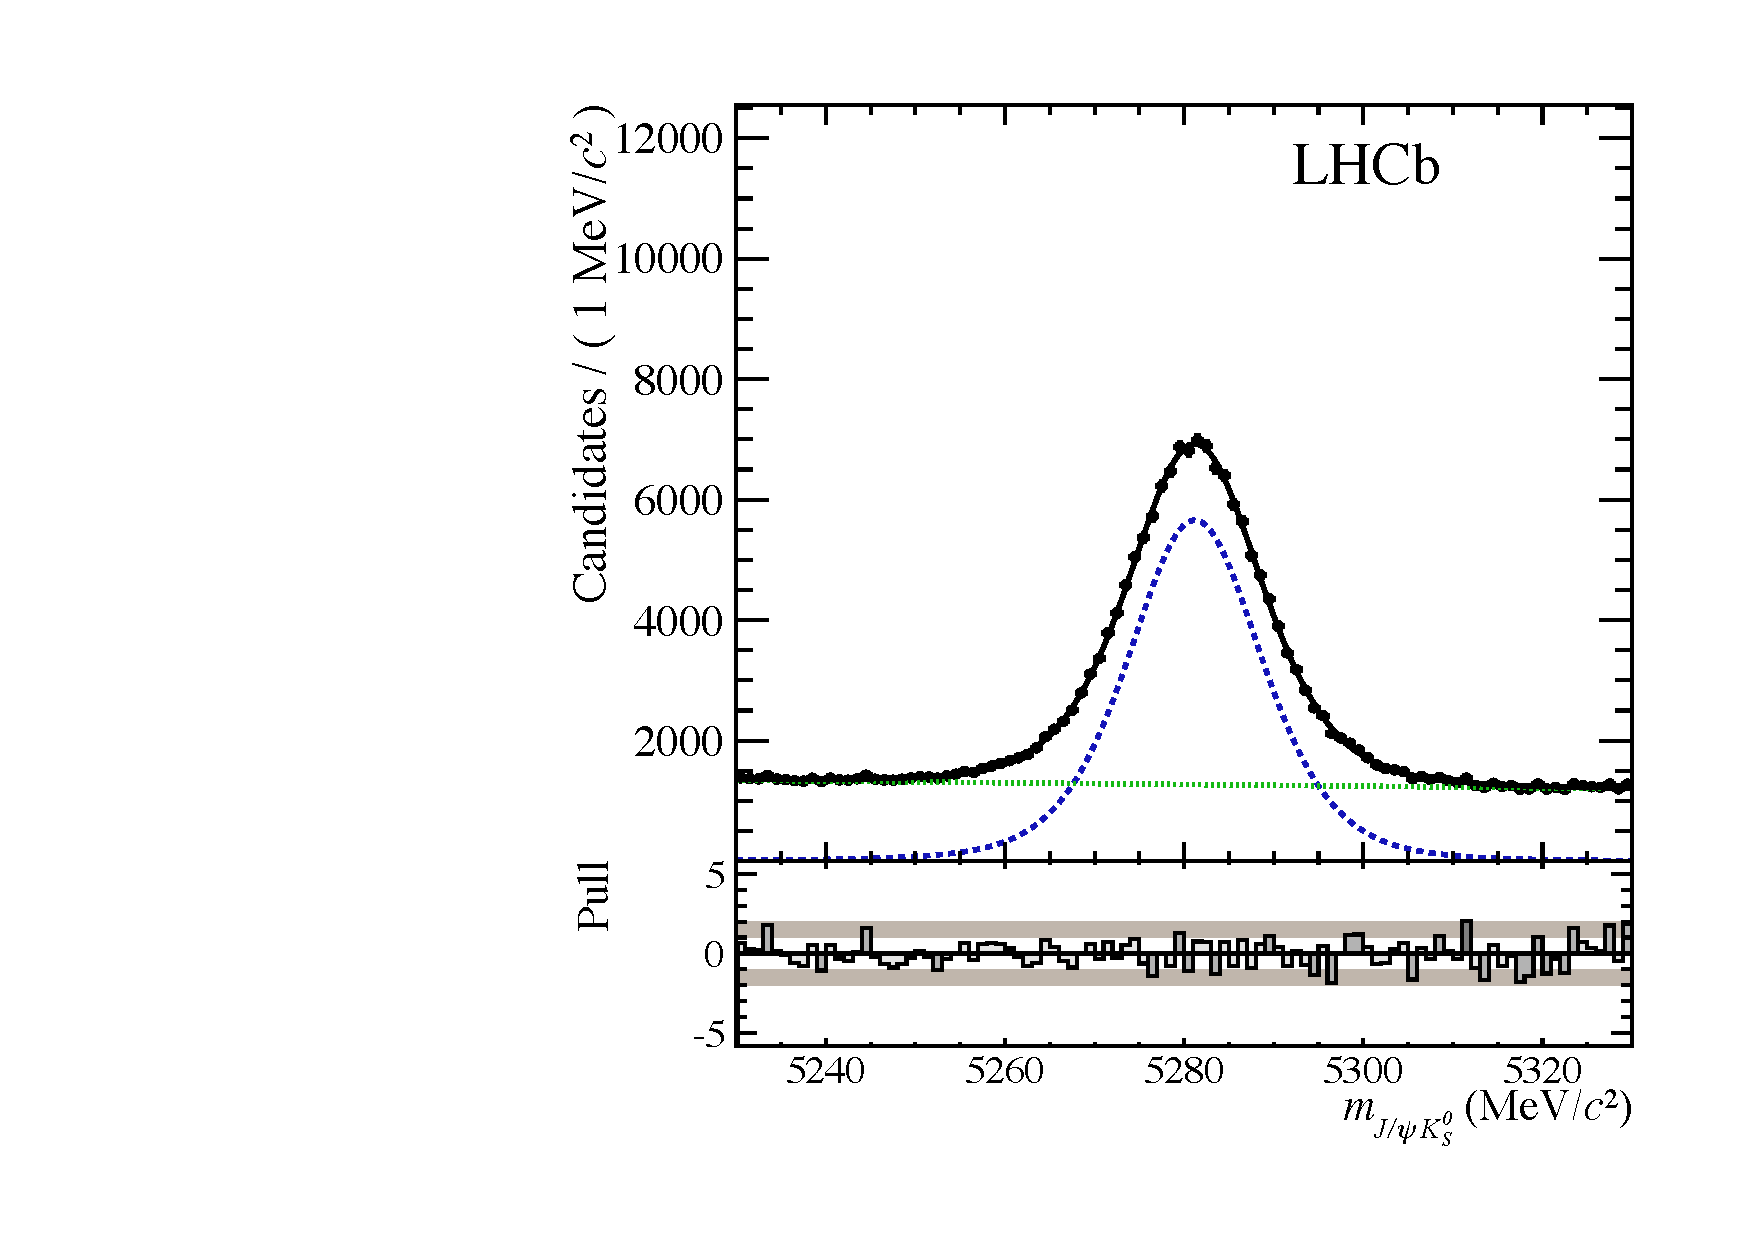
\includegraphics[width=0.49\textwidth]{private/content/measurement-of-sin2beta/figs/mass_trigger_efficiency_biased.pdf}
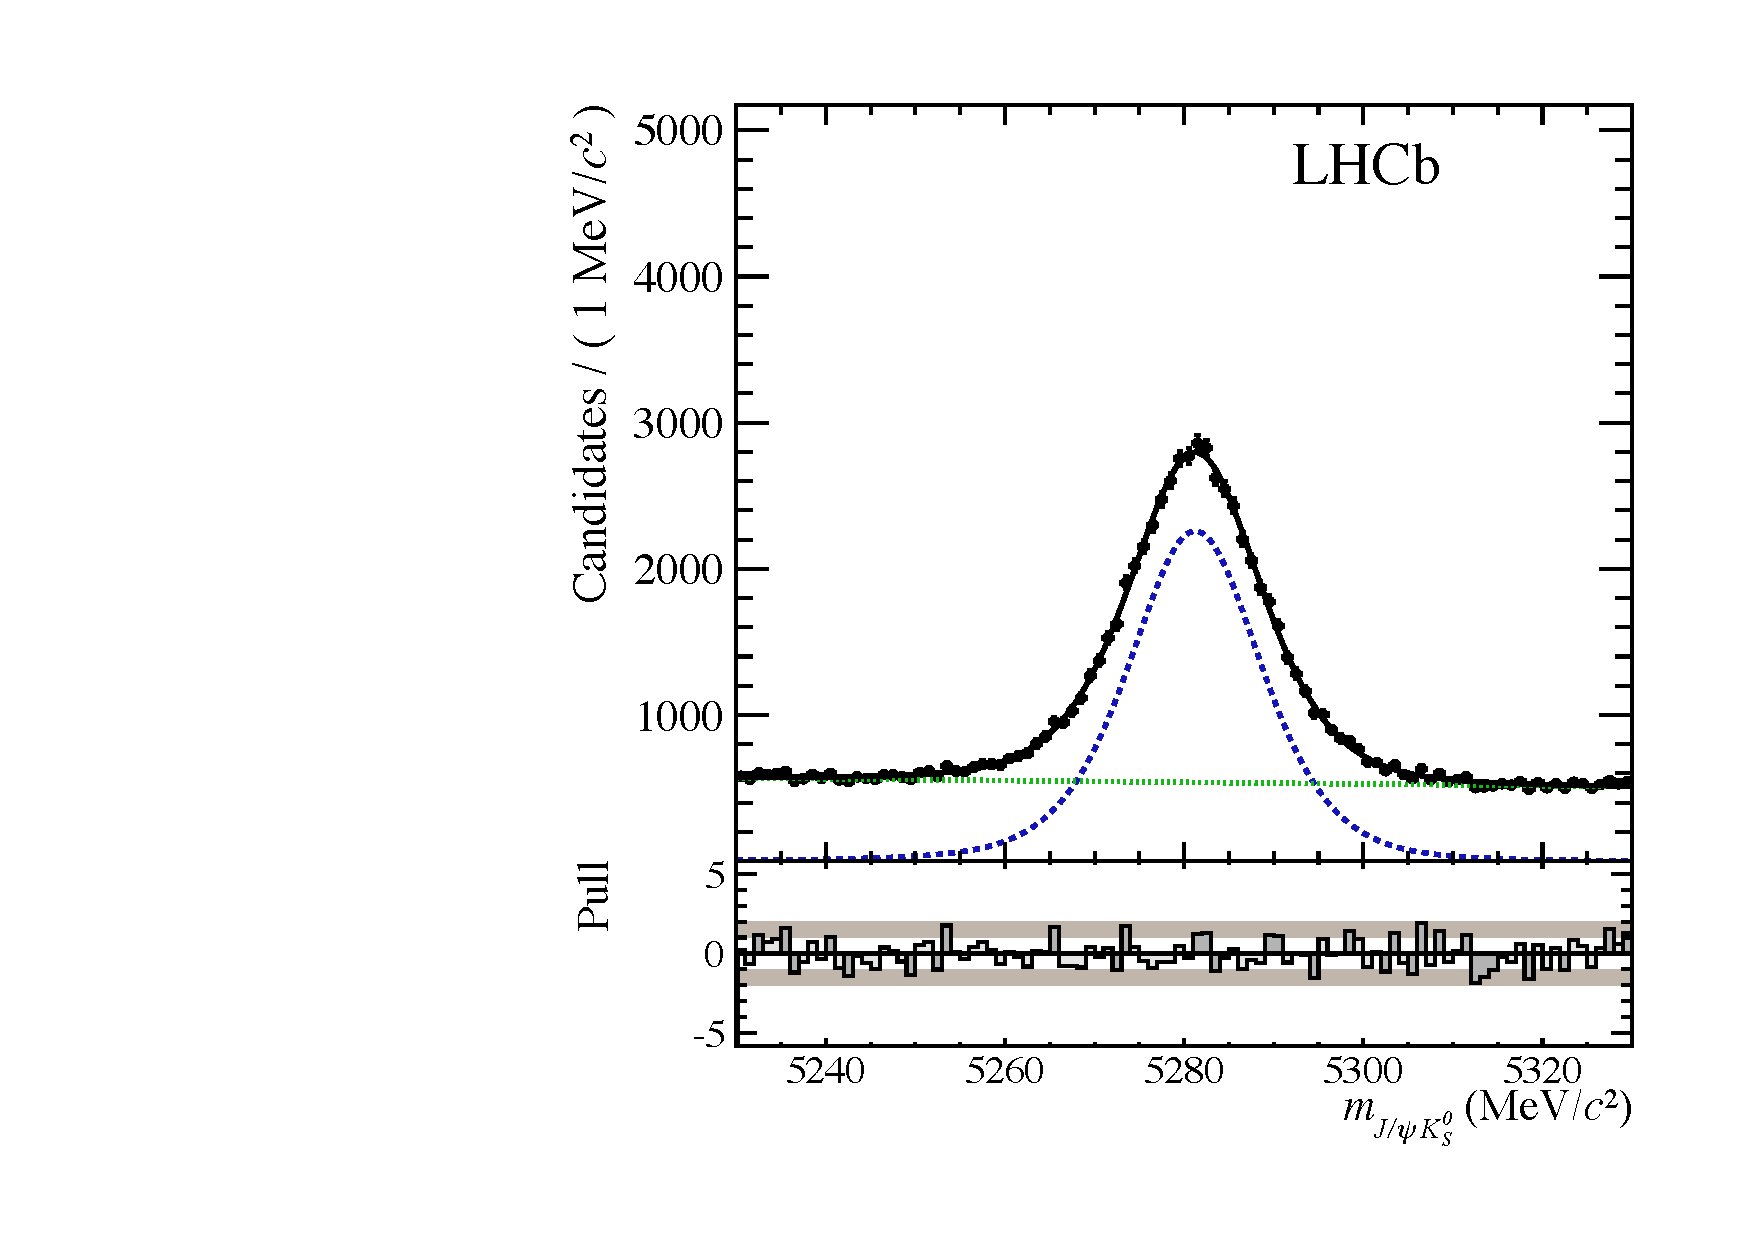
\includegraphics[width=0.49\textwidth]{private/content/measurement-of-sin2beta/figs/mass_trigger_efficiency_unbiased.pdf}
\label{fig:measurement_of_sin2beta:resolution_and_acceptance:acceptance:lower:mass_fits}
\caption{Mass distribution and fit projection summarised over all categories for
the (left) biased (\catAU and \catEB) and the (right) unbiased sample.}
\end{figure}
%
\Cref{fig:measurement_of_sin2beta:resolution_and_acceptance:acceptance:lower:splines} 
shows the acceptance histograms for the almost unbiased and the exclusively
biased sample. In the nominal fit we use cubic splines\addref{Cubic splines}
instead of the histograms themselves. Each bin centre is used as a knot for the
splines. The bin contents determine the shape of the splines. However, the bin
contents aren't fixed but constrained with a Gaussian function where the width
is given by the uncertainty on the bin content. As there is no information about
the acceptance at the decay time limits, the efficiency is assumed to be flat
between the lower decay time limit at \SI{0.3}{\ps} and the first bin
centre/knot and the last bin centre/knot and the upper decay time limit at
\SI{18.3}{\ps}, respectively.
%
\begin{figure}
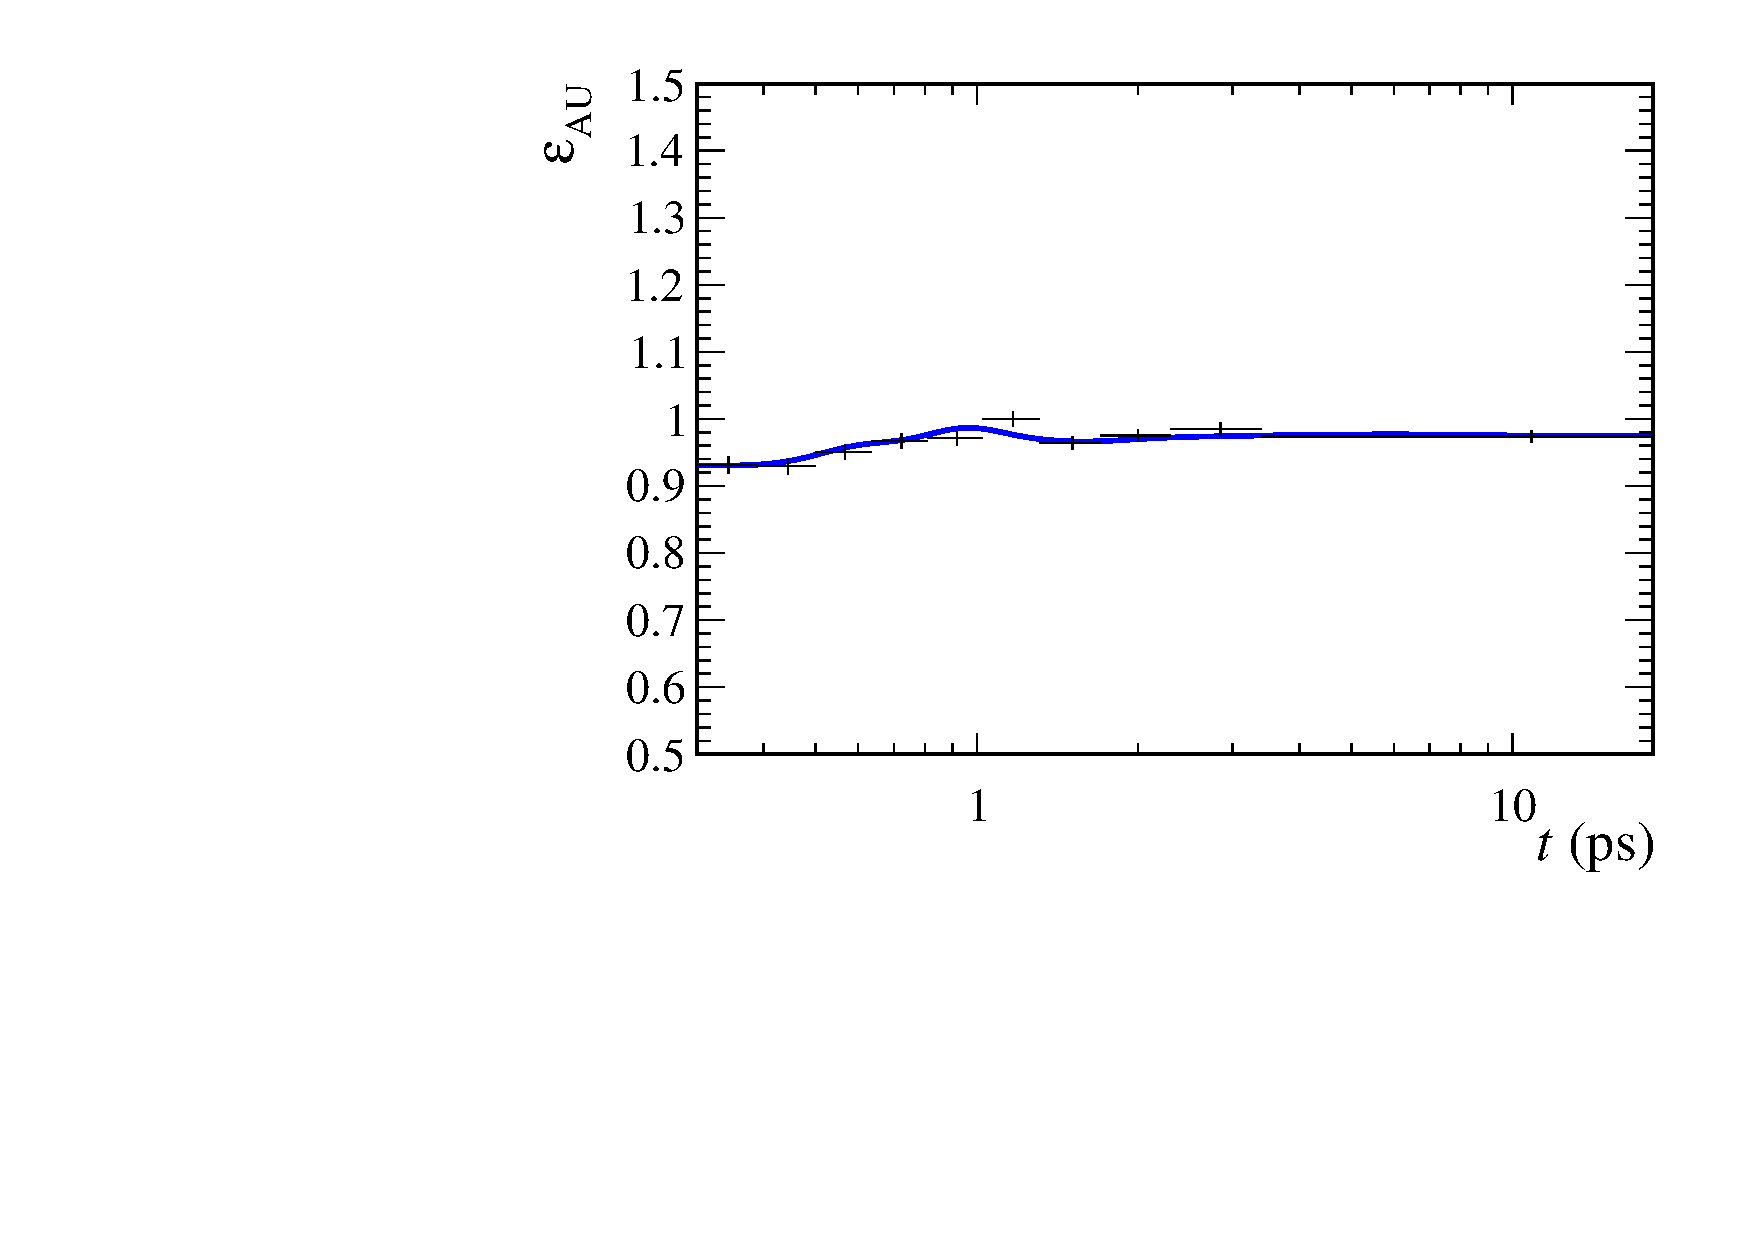
\includegraphics[width=0.49\textwidth]{private/content/measurement-of-sin2beta/figs/trigger_acceptance_spline_AU.pdf}
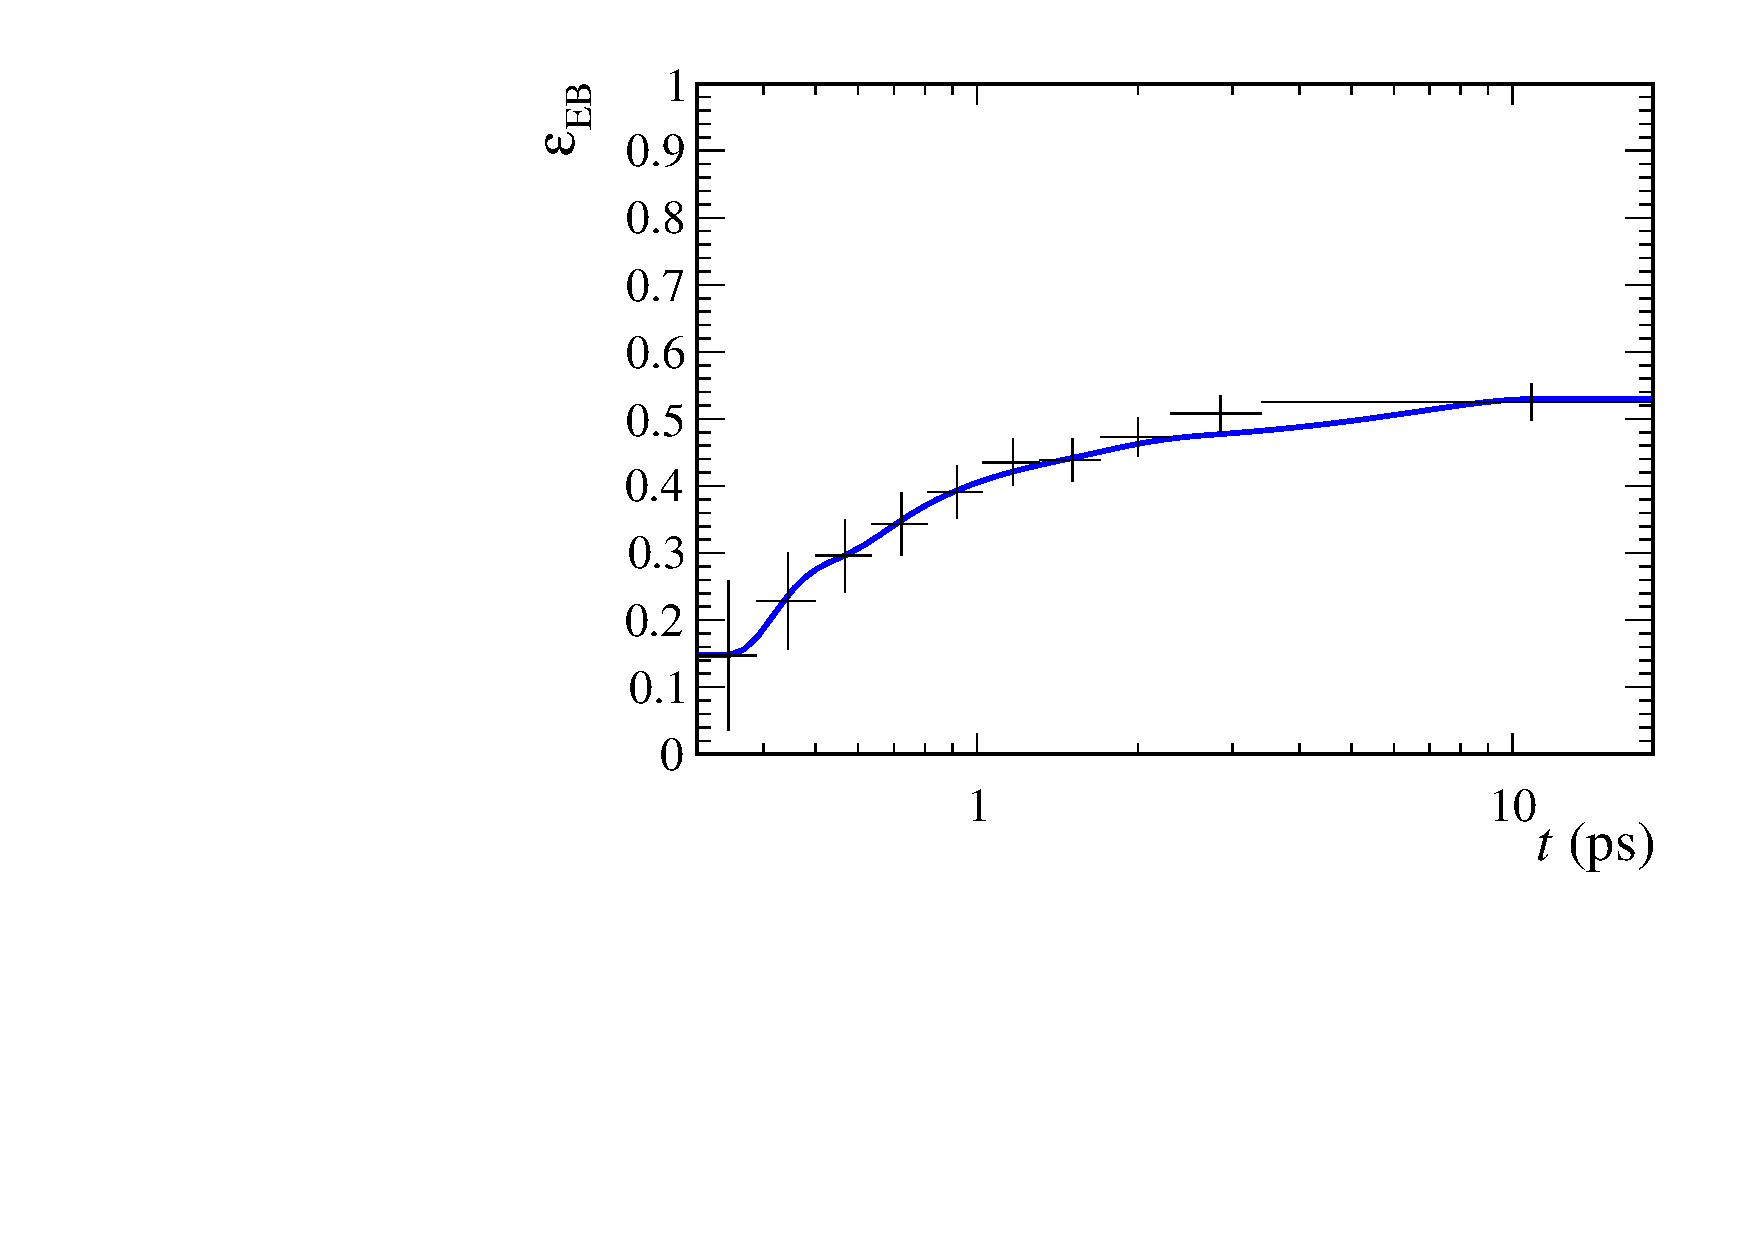
\includegraphics[width=0.49\textwidth]{private/content/measurement-of-sin2beta/figs/trigger_acceptance_spline_EB.pdf}
\label{fig:measurement_of_sin2beta:resolution_and_acceptance:acceptance:lower:splines}
\caption{Histograms of the trigger acceptance for the (left) almost unbiased and
the (right) exclusively biased sample. The blue curve shows the fitted
acceptance using cubic splines.}
\end{figure}

% ..............................................................................
\subsubsection{Upper decay time acceptance}
\label{sec:measurement_of_sin2beta:resolution_and_acceptance:acceptance:upper}

Due to the \VELO reconstruction inefficiency\todo{Be more precise, FastVelo
algorithm} and other reconstruction and selection effects, a decay time
acceptance is observed for events with larger decay times. To account for
this effect a correction factor $\beta_\tau$ is included into the fit model
using the modified lifetime
%
\begin{equation}
  \widetilde{\tau} = \frac{\tau}{1 + \beta_\tau \tau} ,
\end{equation}
%
which expands to
%
\begin{equation}\label{eq:measurement_of_sin2beta:resolution_and_acceptance:acceptance:upper:linear}
\begin{split}
  \Prob{}{}\left(t\right) &= \exponential{-\frac{t}{\tau}\left(1+\beta_{\tau}\tau\right)} \\
                          &= \exponential{-\frac{t}{\tau}-\beta_{\tau}t} = \exponential{-\frac{t}{\tau}} \exponential{-\beta_{\tau}t} \\
                          &= \exponential{-\frac{t}{\tau}}\left(1-\beta_{\tau} t+\frac{\beta_{\tau}^2 t^2}{2}+\order{\left((\beta_{\tau} t)^3\right)}\right).
\end{split}
\end{equation}
%
The value of $\beta_\tau$ is determined using a fit to simulated data while
fixing the lifetime $\tau$ to its generation value. Based on the
\BdToJpsiKS signal \MC data set, only candidates passing the
\StrippingPrescaled stripping line and the unbiased trigger lines
\HLTOneDiMuonHighMass and \HLTTwoDiMuonJpsi are chosen to avoid any
additional lifetime bias for events with short decay times. Only candidates
being matched on \MC as true signal events are considered. The nominal offline
selection is applied and from the remaining multiple (\acs{PV},\Bd) candidate pairs,
one is chosen randomly. To avoid wrong-\acs{PV} associations of the reconstructed
\BdToJpsiKS candidate the true \MC decay time is used in the fit. To reduce the
statistical uncertainties and no deviations of the decay time distributions are
expected all untagged events are included in this study. The number of remaining
\MC candidates available for this study is roughly \num{60000}. Due to
differences in the reconstruction efficiency the $\beta_\tau$ factor is
determined separately for \catOO/\catOT and \catDD/\catLL events
(\cref{tab:measurement_of_sin2beta:resolution_and_acceptance:acceptance:upper}).
%
\begin{table}
  \centering
  \caption{Decay time correction factor $\beta_\tau$ in \si{\per\pico\second}.}
  \begin{tabular}{ccc}
    \toprule
     & 2011 & 2012 \\
    \midrule
    downstream & $0.0036\pm0.0029$ & $0.0084\pm0.0032$ \\
    long track & $0.018\pm0.004$   & $0.035\pm0.005$ \\
    \bottomrule
  \end{tabular}
  \label{tab:measurement_of_sin2beta:resolution_and_acceptance:acceptance:upper}
\end{table}

\subsubsection*{Influence of higher order effects}
\todo{Leave out this possibility?}
To check the influence of higher order terms, a quadratic correction function is
tested where the second order term has an own degree of freedom given by
$\gamma_\tau$,
%
\begin{equation}\label{eq:measurement_of_sin2beta:resolution_and_acceptance:acceptance:upper:quadratic}
  \Prob{}{}\left(t\right) = \exponential{-\frac{t}{\tau}}\left(1-\beta_\tau t+ \gamma_\tau t^2\right).
\end{equation}
%
Again the parameters $\beta_\tau$ and $\gamma_\tau$ are fitted while fixing the
lifetime $\tau$. In \cref{tab:measurement_of_sin2beta:resolution_and_acceptance:acceptance:upper:secondorder} 
the results are listed for \catOO/\catOT and \catDD/\catLL events. To visualise
the effect, the per-bin ratio of the decay time distributions of signal \MC
events to events generated from \ToyMC is calculated and shown in
\cref{fig:measurement_of_sin2beta:resolution_and_acceptance:acceptance:upper}.
The \ToyMC decay time distribution follows an exponential function with the same
lifetime as used in the generation of the signal \MC. As the uncertainties on
$\beta_\tau$ and $\gamma_\tau$ are large and the parameters are strongly
correlated ($\rho>\SI{90}{\percent}$) we stick to the linear model. A possible
bias due to this choice is investigated in
\cref{sec:measurement_of_sin2beta:systematics:systematics:acceptance}.
%
\begin{table}
  \centering
  \caption{Decay time correction factors $\beta_\tau$ (in \si{\per\pico\second})
  and $\gamma_\tau$ (in \si{\per\square\pico\second}).}
  \label{tab:measurement_of_sin2beta:resolution_and_acceptance:acceptance:upper:quadratic}
  \begin{tabular}{ccccc}
    \toprule
     & \multicolumn{2}{c}{2011} & \multicolumn{2}{c}{2012} \\
     & $\beta_\tau$ & $\gamma_\tau$ & $\beta_\tau$ & $\gamma_\tau$ \\
    \midrule
    \catDD & $-0.016\pm0.007$ & $-0.0030\pm0.0008$ & $-0.001\pm0.007$         & $-0.0014\pm0.0009$\\ 
    \catLL & $-0.001\pm0.009$ & $-0.0028\pm0.0012$ & $\phantom{+}0.01\pm0.06$ & $-0.0027\pm0.0008$\\ 
    \bottomrule
  \end{tabular}
\end{table}
%
\begin{figure}
  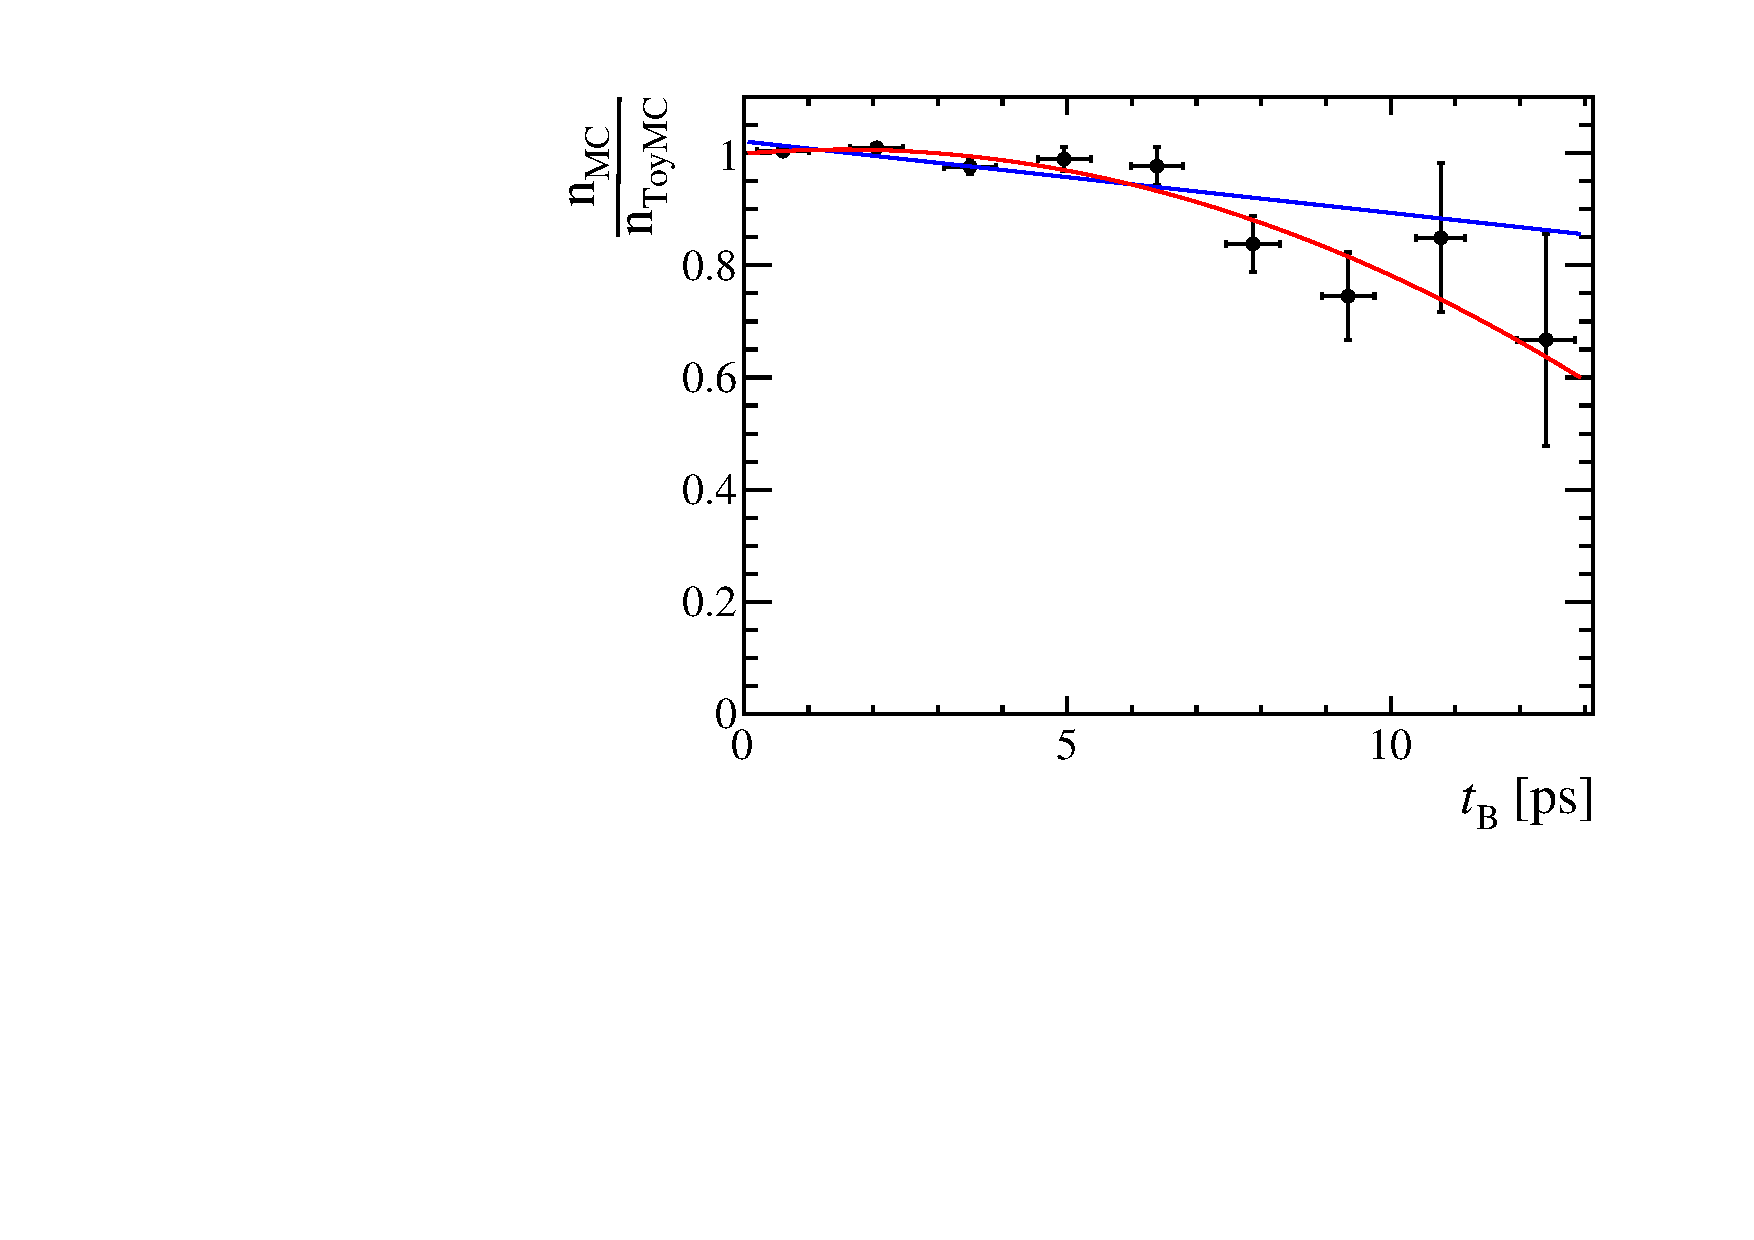
\includegraphics[width=0.49\textwidth]{private/content/measurement-of-sin2beta/figs/velo_acceptance_11_DD.pdf}\hfill
  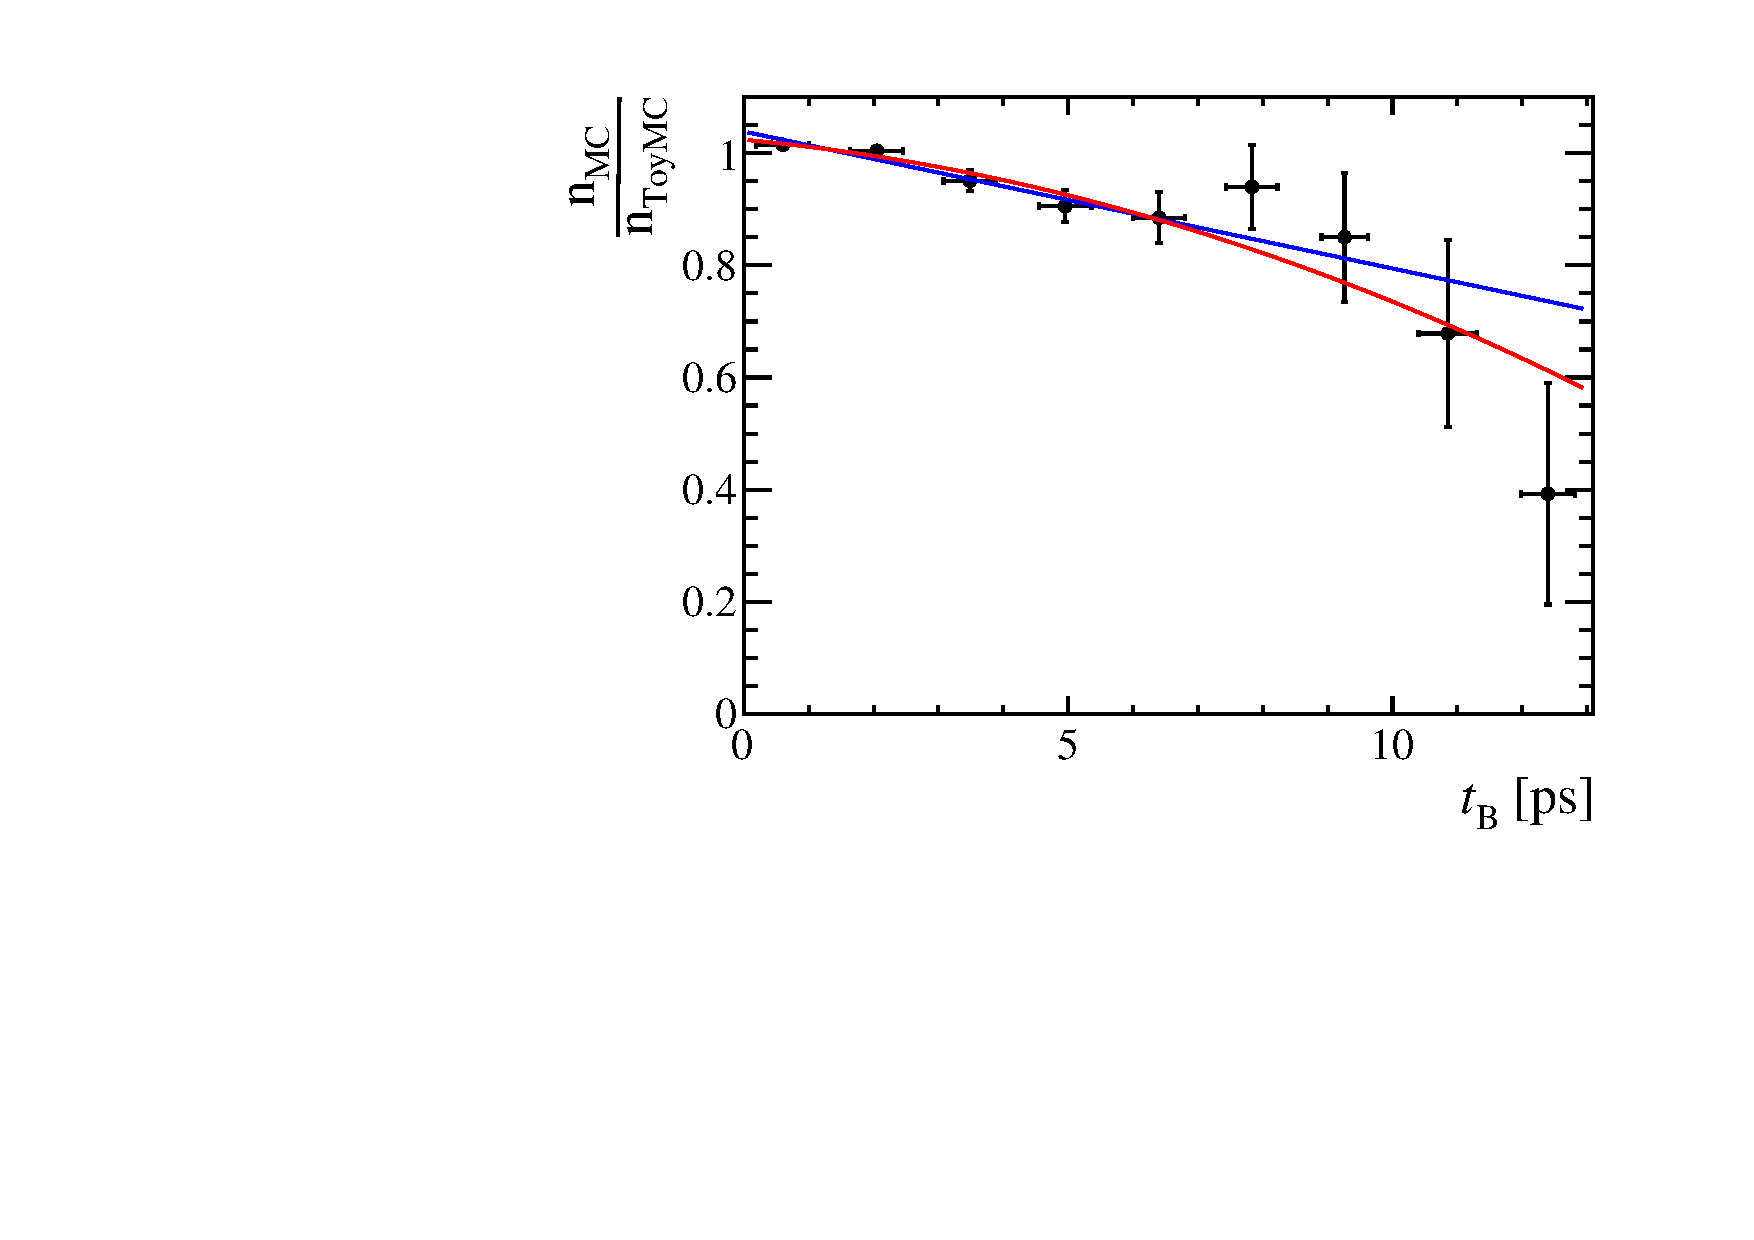
\includegraphics[width=0.49\textwidth]{private/content/measurement-of-sin2beta/figs/velo_acceptance_11_LL.pdf}
  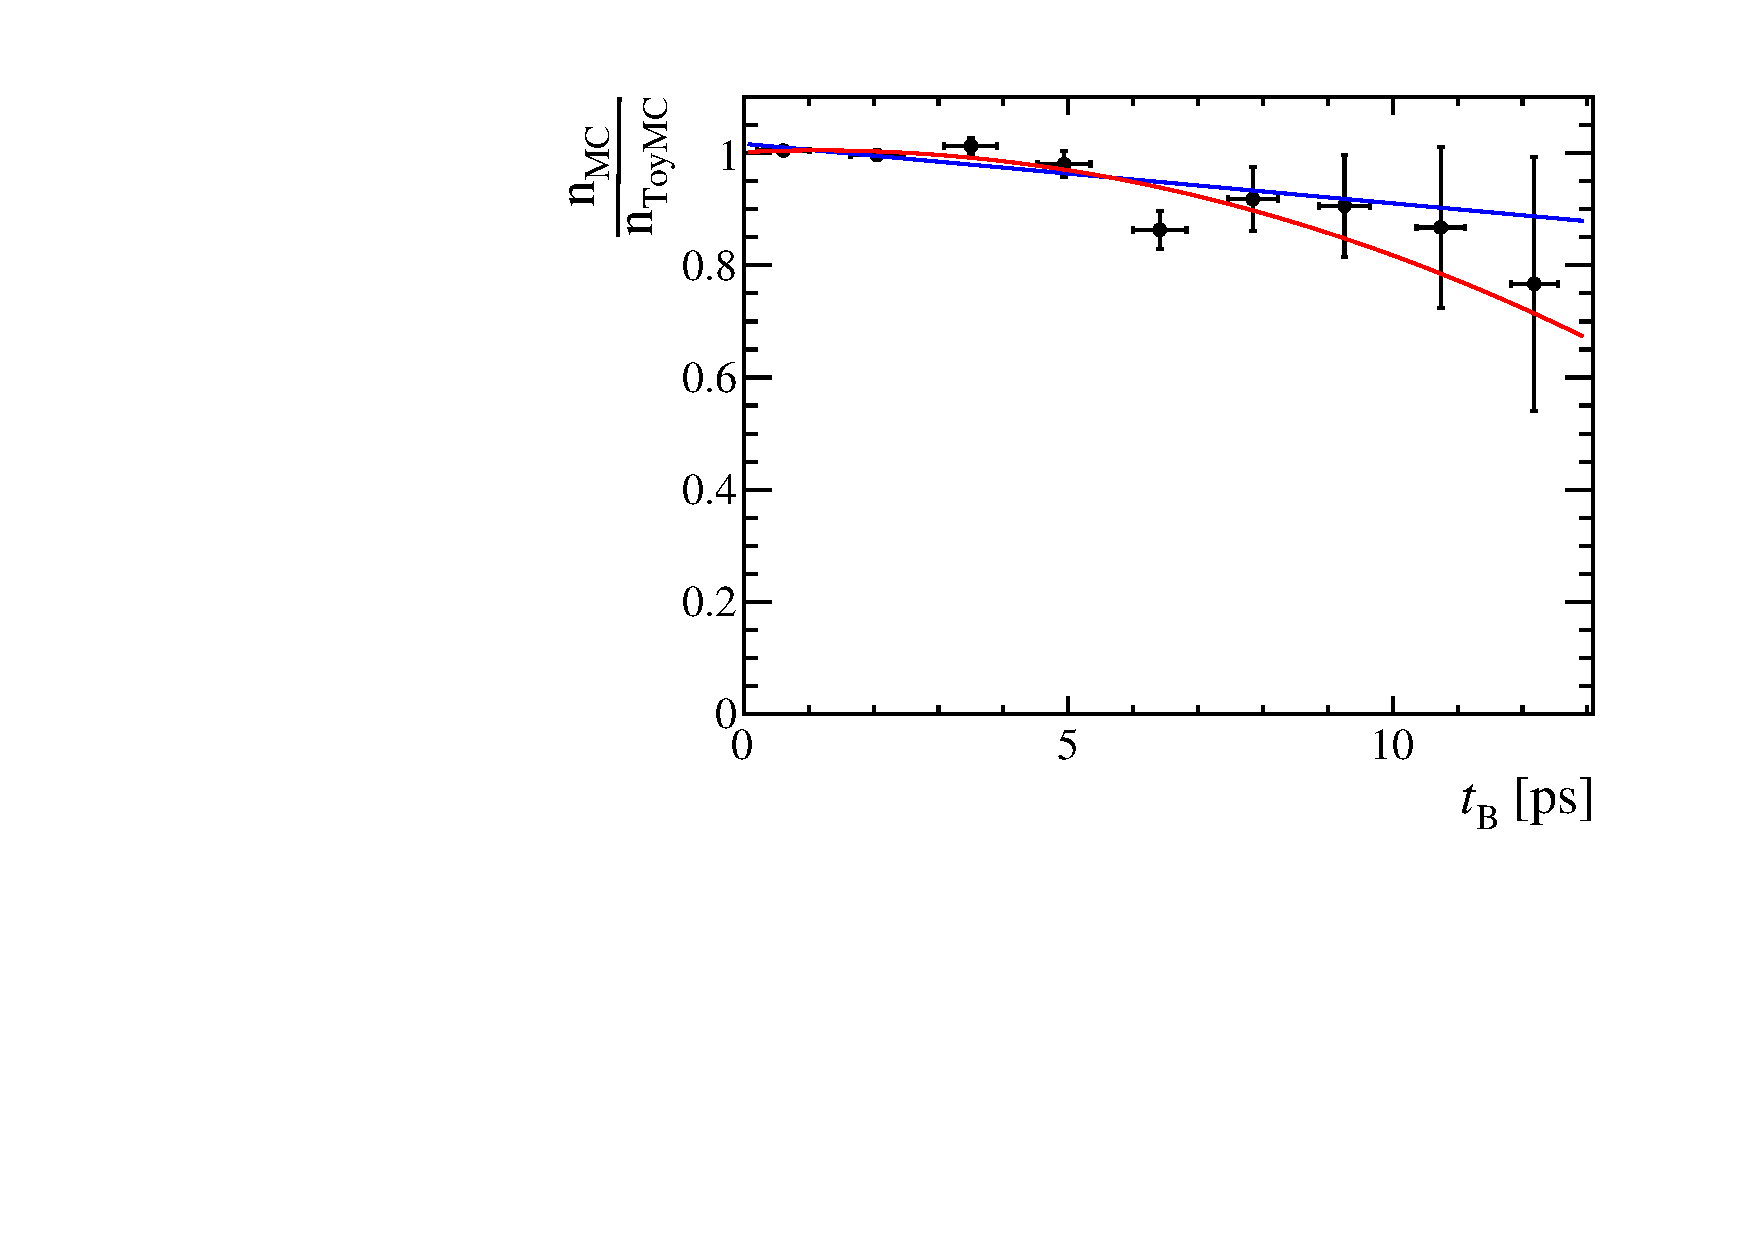
\includegraphics[width=0.49\textwidth]{private/content/measurement-of-sin2beta/figs/velo_acceptance_12_DD.pdf}\hfill
  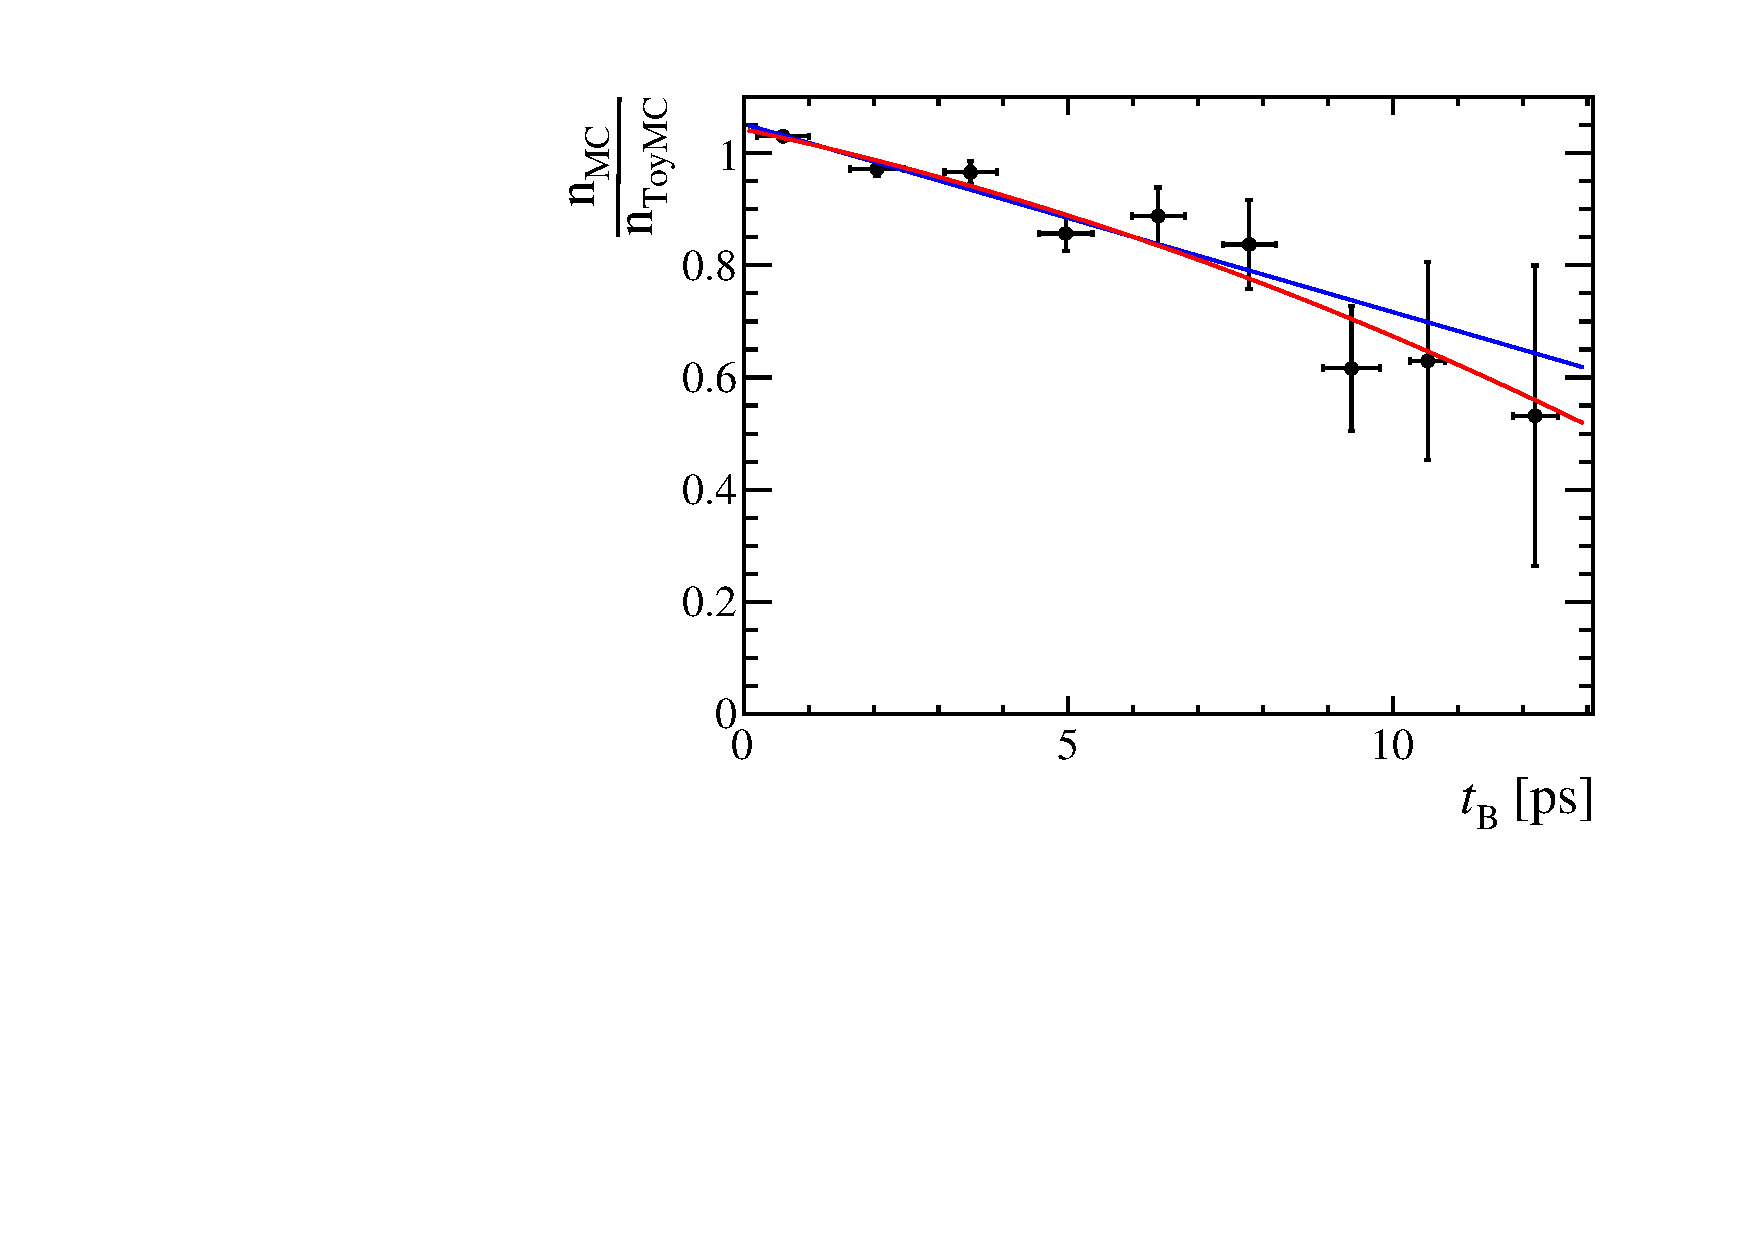
\includegraphics[width=0.49\textwidth]{private/content/measurement-of-sin2beta/figs/velo_acceptance_12_LL.pdf}
\caption{
Decay time ratio in bins of decay time for (left/right) \catDD/\catLL and
(top/bottom) \catOO/\catOT. The blue (red) curve shows a linear (quadratic) fit
to the data points.}
\label{fig:measurement_of_sin2beta:resolution_and_acceptance:acceptance:upper}
\end{figure}
